\documentclass[12pt,a4paper]{article}
\usepackage[utf8]{inputenc}
\usepackage[greek,english]{babel}
\usepackage{alphabeta} 
\usepackage[pdftex]{graphicx}
\usepackage[top=1in, bottom=1in, left=0.5in, right=0.5in]{geometry}
\linespread{1}
\setlength{\parskip}{8pt plus2pt minus2pt}
\widowpenalty 10000
\clubpenalty 10000
\newcommand{\eat}[1]{}
\newcommand{\HRule}{\rule{\linewidth}{0.5mm}}
\usepackage[official]{eurosym}
\usepackage{enumitem}
\setlist{nolistsep,noitemsep}
\usepackage[hidelinks]{hyperref}
\usepackage{cite}
\usepackage{lipsum}
\graphicspath{ {./images/} }
\usepackage{listings}
\usepackage{color}
\setlength{\parindent}{0pt}


\definecolor{dkgreen}{rgb}{0,0.6,0}
\definecolor{gray}{rgb}{0.5,0.5,0.5}
\definecolor{mauve}{rgb}{0.58,0,0.82}


\lstset{frame=tb,
	language=C,
	aboveskip=3mm,
	belowskip=3mm,
	showstringspaces=false,
	columns=flexible,
	basicstyle={\small\ttfamily},
	numbers=none,
	numberstyle=\tiny\color{gray},
	keywordstyle=\color{blue},
	commentstyle=\color{dkgreen},
	stringstyle=\color{mauve},
	breaklines=true,
	breakatwhitespace=true,
	tabsize=3
}


\title{ECE 351 Lab8}
\author{Zachary DeLuca}
\date{March 21st 2023}

\begin{document}
	
\maketitle
\hline
\section{Introduction}
	In this lab we will use the Fourier series  to approximate another function. As it would take an infinite amount of sine or cosine waves to perfectly describe a square wave, we will approximate it using a series of increasing sine waves. In this lab we will show how many sine waves are required to make a square wave or at least a convincing approximation. 

\section{Equations}
$$x(t)=\frac{a_0}{2}+\sum_{k=1}^{\infty}{a_kcos(k\omega_0t)+b_ksin(k\omega_0t)}$$
$$x(t)=\sum_{k=1}^{\infty}{b_ksin(k\omega_0t)}$$
$$b_k=\frac{2}{T}\int_0^T{x(t)sin(k\omega_0t)}dt=\frac{4}{T}\int_0^{T/2}{sin(k\omega_0t)}dt$$
$$b_k=\frac{2}{k\pi}-\frac{4cos(k\omega_0t)}{k\pi}$$
$$b_k=\frac{2}{k\pi}(1+(-1)^k)$$
$$x(t)=\sum_{k=1}^{\infty}{\frac{2}{k\pi}(1+(-1)^k)sin(k\omega_0t)}$$

\section{Graph}
Using python we can add a finite amount of sine waves using the formula above. Below are displayed the result when there were 1 term, 3 terms, 15 terms, 50 terms, 150 terms, and 1500 terms. \vspace{12pt}

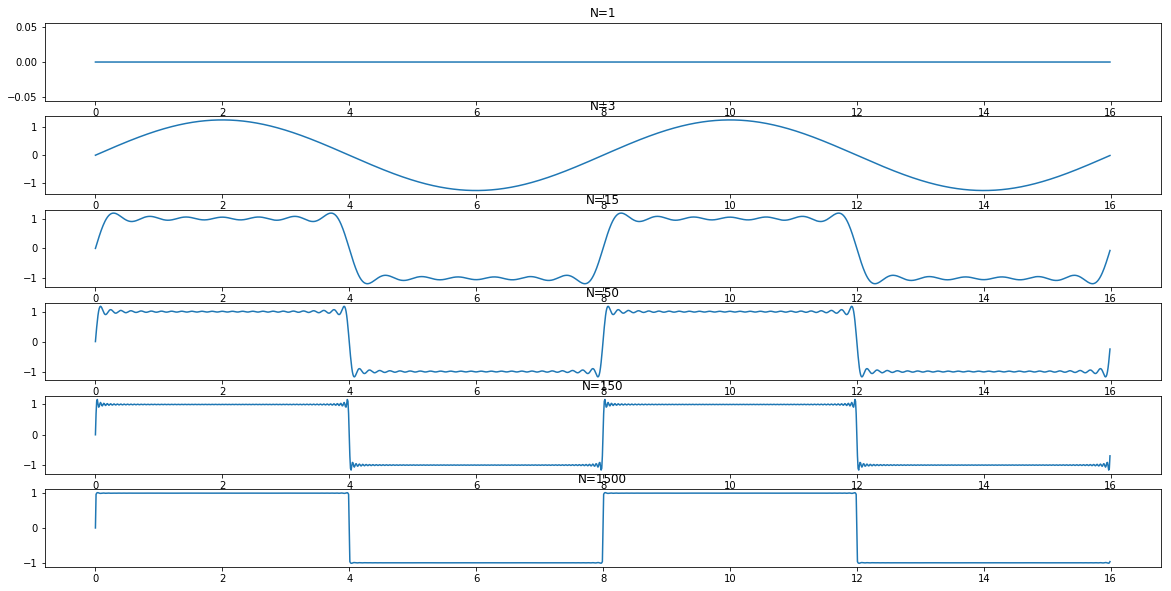
\includegraphics[width=\linewidth]{/home/zachariahmus/Documents/Code_Projects/351Lab8/Lab8/ResultGraph.PNG}

As we expect, the more terms that are added yield a clearer square wave
\section{Post Lab Questions}

	1. Is x(t) an even or an odd function? Explain why.\vspace{6pt}
		
	     It is an odd function because it does not mirror across the y axis, but does mirror over y=x.\vspace{6pt}
		
	2. Based on your results from Task 1, what do you expect the values of a2, a3, . . . , an to be?
	Why?\vspace{6pt}
	
	     The values for A are always 0 as it is an odd function. If we were to evaluate, we would always find the sin or cos term at some integer multiple of an angle that yielded 0. \vspace{6pt}
	
	3. How does the approximation of the square wave change as the value of N increases? In what
	way does the Fourier series struggle to approximate the square wave?\vspace{6pt}
	
	     As the value of N increases, the square-wave becomes more and more apparent and more defined. The corners are the last thing to be shaped by the increasing terms.\vspace{6pt}  
	
	4. What is occurring mathematically in the Fourier series summation as the value of N increases?\vspace{6pt}
	
	     The summation is adding increasingly small new sine waves to the current waveform in order to shape it more accurately and precisely into the waveform it is meant to model. \vspace{6pt}



\section{Conclusion}
	In this lab we were able to create a square wave using sine waves with the Fourier series. Using computers to aid the process that would be somewhere between tedious and impossible for a human to do we were able to graphically show what the Fourier series does mathematically. The square wave was simple enough that this was good demonstration, and its application for more varied periodic signals can be extrapolated and understood. 
	
\end{document}
